\section{Introduction}

Nowadays, it is common for players to play cooperative games from different country under highly developed Internet environment. 
In our pilot study, we observed that playing cooperative game, which required high-level-feature communication, with different language speaker would cause frustrating game experience.

We suggest to use body language as a communication manner in cooperative game to get better game experience. With this approach, no matter playing with different language speaker or common language speaker, player would have consistent game experience. 

We also provide a game prototype, Mute Robot, to explore cooperative game design through body language. Mute Robot provides three game stages for players to solve puzzles.
To encourage players to use body language, we have designed an asymmetric puzzle system, with only one player receiving puzzle hints. The player will use body language to guide the other player to solve the puzzle.

By using extended Short Feedback Questionnaire (eSFQ)\cite{eSFQ} and Cooperative Performance Metrics (CPMs)\cite{CPMs} to evaluate game experience, our user study results indicate that, using body language in cooperative game design would enhance original game experience and decrease 48\% frustrating caused by language boundary. And we observe that cooperative game has consistent game experience with body language communication.

% According to our final questionnaire, only 17\% and 25\% (different language group and common language group) player choose traditional communication manner (speaking) as the favorite manner.
According to our final questionnaire, after adding the communication manner of body language, 83\% and 75\% (different language group and common language group) players choose our new communication manner (``body language'' and ``both'') as the favorite manner. 

We also observe some interesting communication patterns. Game developer can make a better game experience with these information. We hope to inspire more exploration of using body language in game designs and spread game entertainment for more people.


\begin{figure}[t]
\centering
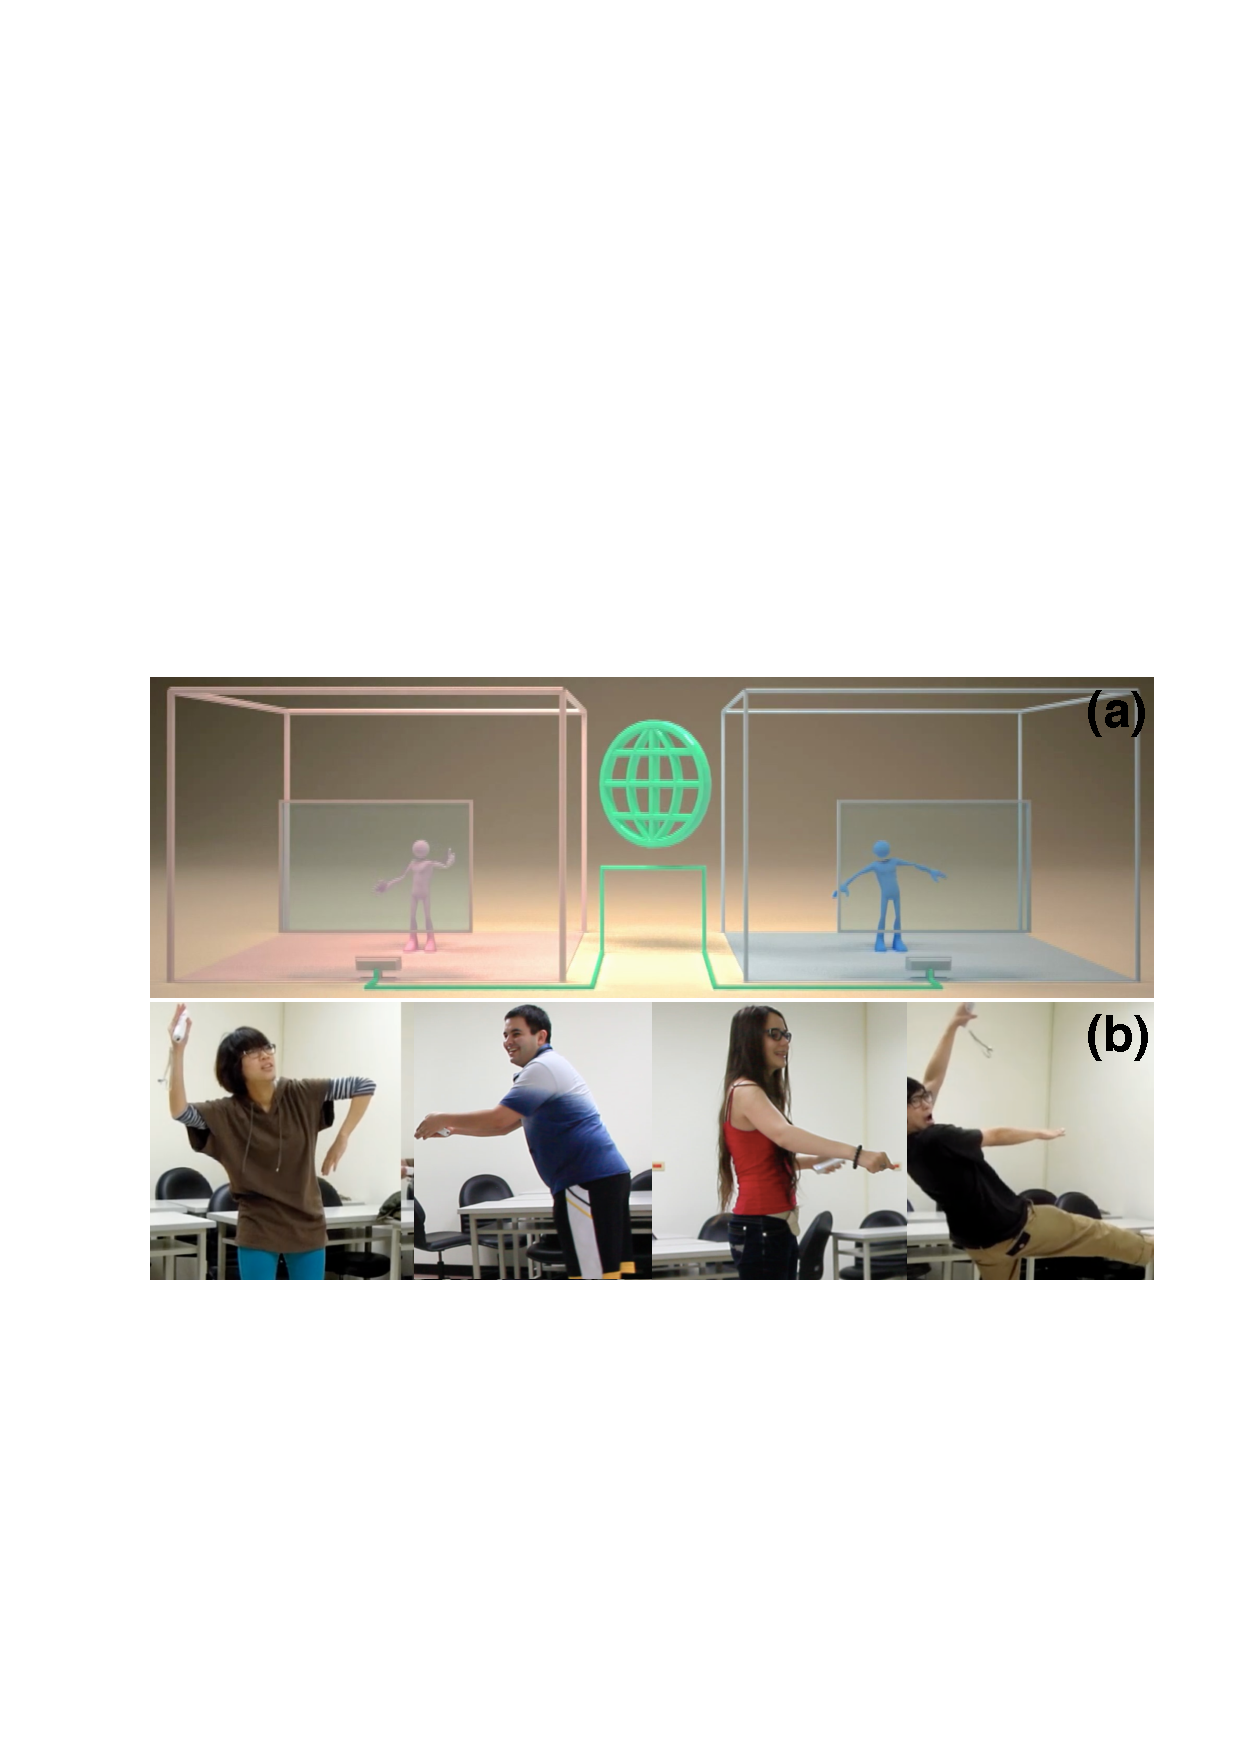
\includegraphics[width=0.9\columnwidth]{Figures/Topic.pdf}
\caption{(a) Playing cooperative games via Internet, (b) Using body language as a communication manner}
\label{fig:Topic}
\end{figure}

